\documentclass{standalone}
\usepackage{tikz}
\usetikzlibrary{shapes.geometric, arrows.meta}

\tikzset{
    state/.style={rectangle, rounded corners, minimum width=3cm, minimum height=1cm, text centered, draw=black, fill=red!30},
    observation/.style={circle, minimum size=1cm, text centered, draw=black, fill=blue!30},
    action/.style={rectangle, minimum width=2cm, minimum height=1cm, text centered, draw=black, fill=green!30},
    arrow/.style={thick,->,>=stealth}
}

\begin{document}
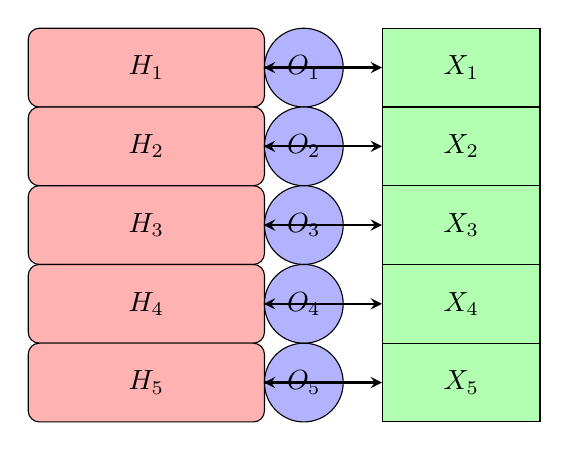
\begin{tikzpicture}[node distance=2cm]

    % Hidden States
    \foreach \i in {1,...,5} {
        \node[state] (H\i) at (0,-\i) {$H_\i$};
    }

    % Observations
    \foreach \i in {1,...,5} {
        \node[observation] (O\i) at (2,-\i) {$O_\i$};
    }

    % Actions
    \foreach \i in {1,...,5} {
        \node[action] (X\i) at (4,-\i) {$X_\i$};
    }

    % Arrows between nodes
    \foreach \i in {1,...,4} {
        \draw [arrow] (H\i) -- (O\i);
        \draw [arrow] (H\i) -- (X\i);
    }
    \draw [arrow] (H5) -- (O5);
    \draw [arrow] (H5) -- (X5);

\end{tikzpicture}
\end{document}